\documentclass[aspectratio=43]{beamer}
\usepackage[english]{babel}
% \usepackage[linesnumbered, ruled, vlined]{algorithm2e}
\usepackage{algorithm,algpseudocode}
\usepackage{amsthm}
\usepackage{mathtools}
\usepackage{physics}
\usepackage{calligra}
\usepackage{csquotes}
\usepackage{tensor}
\usepackage[thicklines]{cancel}
\usepackage{tcolorbox}
\usepackage{pstricks}
\usepackage[backend=biber, bibstyle=nature, sorting=nty, citestyle=numeric-comp]{biblatex} %Custom bibliography
% \addbibresource{bib.bib} %Load references


\DeclareMathAlphabet{\mathcalligra}{T1}{calligra}{m}{n}
\DeclareFontShape{T1}{calligra}{m}{n}{<->s*[2.2]callig15}{}
\newcommand{\scriptr}{\mathcalligra{r}\,}
\newcommand{\boldscriptr}{\pmb{\mathcalligra{r}}\,}
\def\rc{\scriptr}
\def\brc{\boldscriptr}
\def\hrc{\hat\brc}
\newcommand{\ie}{\emph{i.e.}} %id est
\newcommand{\eg}{\emph{e.g.}} %exempli gratia
\newcommand{\rtd}[1]{\ensuremath{\left\lfloor #1 \right\rfloor}}
\newcommand{\dirac}[1]{\ensuremath{\delta \left( #1 \right)}}
\newcommand{\diract}[1]{\ensuremath{\delta^3 \left( #1 \right)}}
\newcommand{\e}{\ensuremath{\epsilon_0}}
\newcommand{\m}{\ensuremath{\mu_0}}
\newcommand{\V}{\ensuremath{\mathcal{V}}}
\newcommand{\prnt}[1]{\ensuremath{\left(#1\right)}} %parentheses
\newcommand{\colch}[1]{\ensuremath{\left[#1\right]}} %square brackets
\newcommand{\chave}[1]{\ensuremath{\left\{#1\right\}}}  %curly brackets

\useoutertheme{infolines}
\useinnertheme{rectangles}
\usefonttheme{professionalfonts}


\definecolor{orange}{HTML}{f28165}
\definecolor{gray}{HTML}{303030}
\definecolor{yellow}{HTML}{f0be52}
\definecolor{lightorange}{HTML}{f19e58}
\definecolor{green_custom}{HTML}{279856}


\renewcommand{\CancelColor}{\color{orange}}

\makeatletter
\newcommand{\mybox}[1]{%
  \setbox0=\hbox{#1}%
  \setlength{\@tempdima}{\dimexpr\wd0+13pt}%
  \begin{tcolorbox}[colback=orange,colframe=orange,boxrule=0.5pt,arc=4pt,
      left=6pt,right=6pt,top=6pt,bottom=6pt,boxsep=0pt,width=\@tempdima]
    \textcolor{white}{#1}
  \end{tcolorbox}
}
\makeatother


\usecolortheme[named=orange]{structure}
\usecolortheme{sidebartab}
\usecolortheme{orchid}
\usecolortheme{whale}
\setbeamercolor{alerted text}{fg=yellow}
\setbeamercolor{block title alerted}{bg=alerted text.fg!90!black}
\setbeamercolor{block title example}{bg=lightorange!60!black}
\setbeamercolor{background canvas}{bg=gray}
\setbeamercolor{normal text}{bg=gray,fg=white}

% \usecolortheme[named=green_custom]{structure}

\setbeamertemplate{footline}[frame number]
        {
    %   \leavevmode%
    %   \hbox{%
    %   \begin{beamercolorbox}[wd=.333333\paperwidth,ht=2.25ex,dp=1ex,center]{author in head/foot}%
    %     \usebeamerfont{author in head/foot}\insertshortauthor~~(\insertshortinstitute)
    %   \end{beamercolorbox}%
    %   \begin{beamercolorbox}[wd=.333333\paperwidth,ht=2.25ex,dp=1ex,center]{title in head/foot}%
    %     \usebeamerfont{title in head/foot}\insertshorttitle
    %   \end{beamercolorbox}%
    %   \begin{beamercolorbox}[wd=.333333\paperwidth,ht=2.25ex,dp=1ex,center]{date in head/foot}%
    %     \usebeamerfont{date in head/foot}\insertshortdate{}%\hspace*{2em}

    % %#turning the next line into a comment, erases the frame numbers
    %     %\insertframenumber{} / \inserttotalframenumber\hspace*{2ex} 

    %   \end{beamercolorbox}}%
    %   \vskip0pt%
    }


\setbeamertemplate{blocks}[rectangle]
\setbeamercovered{dynamic}

\setbeamertemplate{section page}
{
	\begin{centering}
		\begin{beamercolorbox}[sep=27pt,center]{part title}
			\usebeamerfont{section title}\insertsection\par
			\usebeamerfont{subsection title}\insertsubsection\par
		\end{beamercolorbox}
	\end{centering}
}

\setbeamertemplate{subsection page}
{
	\begin{centering}
		\begin{beamercolorbox}[sep=12pt,center]{part title}
			\usebeamerfont{subsection title}\insertsubsection\par
		\end{beamercolorbox}
	\end{centering}
}

\newcommand{\hlight}[1]{\colorbox{violet!50}{#1}}
\newcommand{\hlighta}[1]{\colorbox{red!50}{#1}}
\title{
    Comparison between several \\
    denoising methods for \\ 
    image processing 
} %->->->->-> Check hyperref title <-<-<-<-<-
% \subtitle{And Some Things About It}
\author{
    \href{https://github.com/akhaten}{Jessy Khafif}
}

% \date{Toulouse, 2023}

% \institute[UT3]{
%     UT3 Paul Sabatier%
%     % \\%
%     % University of São Paulo%
% } %You can change the Institution if you are from somewhere else
% % \date{February 31, 2019}
% % \logo{
\includegraphics[width= 0.3\textwidth]{images/ut3_logo.png}}

\begin{document}
    
    \frame{\titlepage}
    
    \begin{frame}{Summary}
        \tableofcontents
    \end{frame}
    
    % \input{chapters/a-silly-idea.tex} %You can put the frames directly into the presentation, but using the input command and writing them in separate .tex files might be more organized
    
    \section{Non Local Mean (NLM)}
\frame{\sectionpage}
    
    % \begin{frame}{Ordinary Differential Equations}
    %     \uncover<+->{\begin{equation*}
    %         \dv{x} y(x) + \frac{1}{CR} y(x) = 0
    %     \end{equation*}}
        
    %     \uncover<+->{\begin{equation*}
    %         \dv[2]{x} y(x) + \gamma \dv{x} y(x) + \omega_0^2 y(x) = f(x)
    %     \end{equation*}}
    % \end{frame}
    
    % \begin{frame}{Livin' La Vida Loca}
    %     \uncover<+>{\begin{equation*}
    %         \dv[2]{x} y(x) + \gamma \dv{x} y(x) + \omega_0^2 y(x) = f(x)
    %     \end{equation*}}
    %     \uncover<+>{\[ \Downarrow \]
    %     \begin{equation*}
    %         \colch{\dv[2]{x} + \gamma \dv{x} + \omega_0^2} y(x) = f(x)
    %     \end{equation*}}
    %     \uncover<+>{\[ \Downarrow \]
    %     \begin{equation*}
    %         y(x) = \frac{f(x)}{\dv[2]{x} + \gamma \dv{x} + \omega_0^2}
    %     \end{equation*}}
    % \end{frame}
    
    % \begin{frame}{Livin' La Vida Loca}
    %     \centering
    %     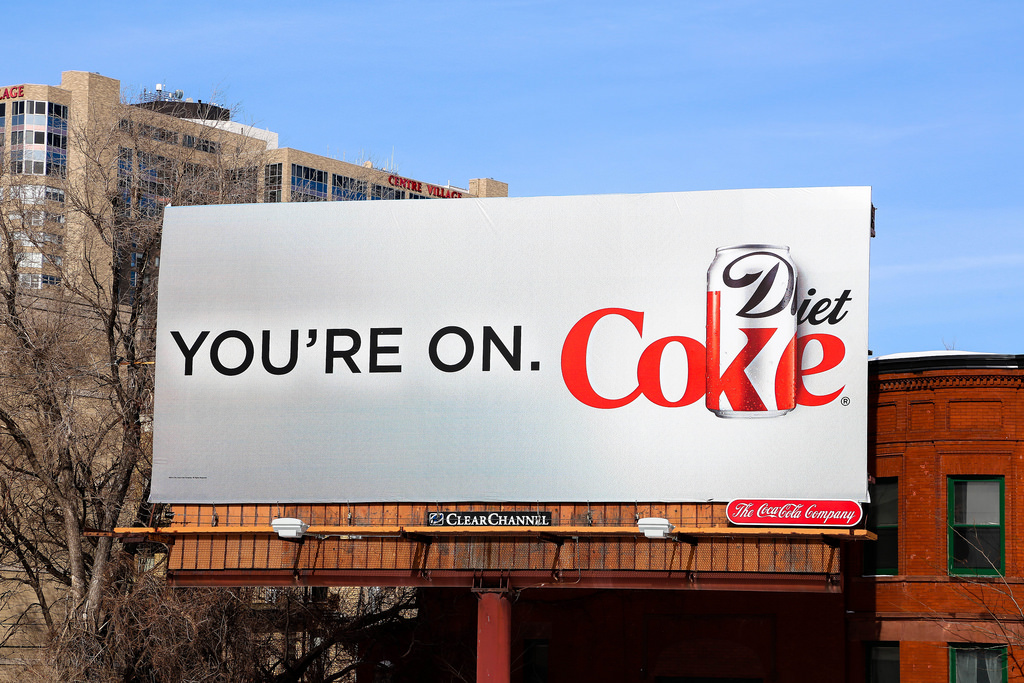
\includegraphics[width = 0.8\textwidth]{images/coke.jpg}
    % \end{frame}
    
    % \begin{frame}{Pandora's Box}
    %     \centering
    %     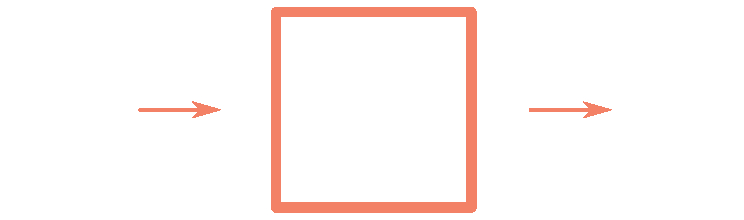
\includegraphics[width = 0.9\textwidth]{images/fourier-1.pdf}
    % \end{frame}
    
    % \begin{frame}{Pandora's Box}
    %     \centering
    %     
\includegraphics[width = 0.9\textwidth]{images/fourier-2.pdf}
    % \end{frame}
    
    % \begin{frame}{Pandora's Box}
    %     \centering
    %     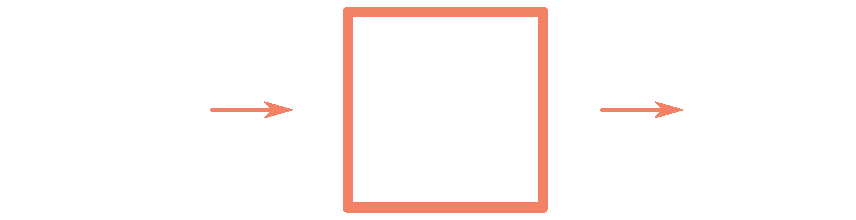
\includegraphics[width = 0.9\textwidth]{images/fourier-3.pdf}
    % \end{frame}
    
    % \begin{frame}{Pandora's Box}
    %     \centering
    %     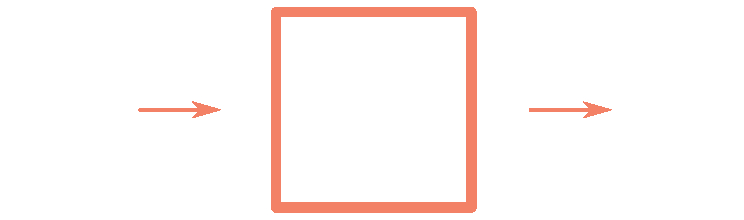
\includegraphics[width = 0.9\textwidth]{images/fourier-4.pdf}
    % \end{frame}
    
    % \begin{frame}{Pandora's Box}
    %     \centering
    %     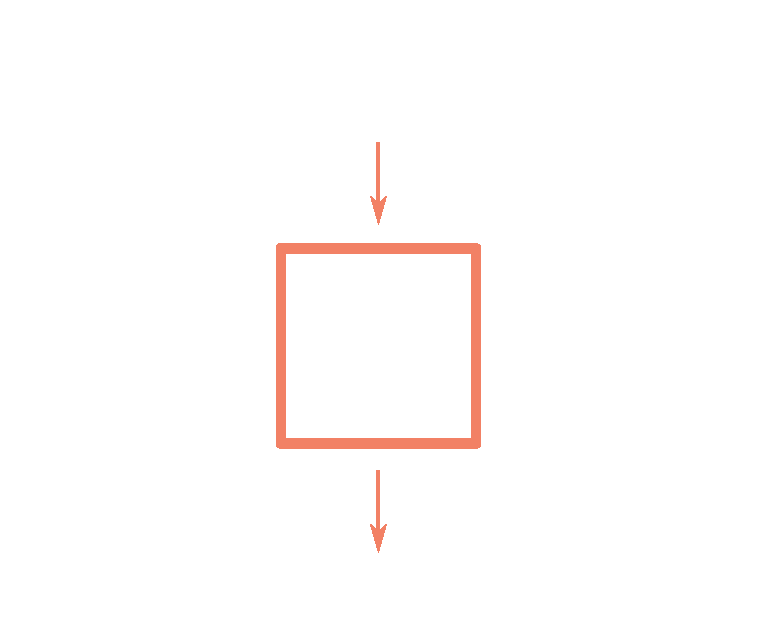
\includegraphics[height = 0.7\textheight]{images/fourier-5.pdf}
    % \end{frame}
    
    % \begin{frame}{Box Proposal}
    %     \uncover<+>{\begin{equation*}
    %         \mathcal{F}[f](\xi) = \hat{f}(\xi) = \frac{1}{\sqrt{2\pi}} \int_{-\infty}^{+\infty} f(x) e^{-i x \xi} \dd{x}
    %     \end{equation*}}
    %     \uncover<+>{\begin{equation*}
    %         \mathcal{F}^{-1}[\hat{f}](x) = f(x) = \frac{1}{\sqrt{2\pi}} \int_{-\infty}^{+\infty} \hat{f}(\xi) e^{i x \xi} \dd{\xi}
    %     \end{equation*}}
    % \end{frame}
    
    % \begin{frame}{Quality Control}
    %     \uncover<+>{\begin{equation*}
    %         \widehat{(f + \alpha g)}(\xi) = \frac{1}{\sqrt{2\pi}} \int_{-\infty}^{+\infty} \prnt{f(x) + \alpha g(x)} e^{-i x \xi} \dd{x}
    %     \end{equation*}}
    %     \uncover<+>{\[ \Downarrow \]
    %     \begin{equation*}
    %         \widehat{(f + \alpha g)}(\xi) = \frac{1}{\sqrt{2\pi}} \int_{-\infty}^{+\infty} f(x) e^{-i x \xi} \dd{x} + \frac{\alpha}{\sqrt{2\pi}} \int_{-\infty}^{+\infty} g(x) e^{-i x \xi} \dd{x}
    %     \end{equation*}}
    %     \uncover<+>{\[ \Downarrow \]
    %     \begin{equation*}
    %         \widehat{(f + \alpha g)}(\xi) = \hat{f}(\xi) + \alpha \hat{g}(\xi)
    %     \end{equation*}}
    % \end{frame}
    
    % \begin{frame}{Quality Control}
    %     \uncover<+>{\begin{equation*}
    %         \widehat{f'}(\xi) = \frac{1}{\sqrt{2\pi}} \int_{-\infty}^{+\infty} f'(x) e^{-i x \xi} \dd{x}
    %     \end{equation*}}
    %     \uncover<+>{\[ \Downarrow \]
    %     \begin{equation*}
    %         \widehat{f'}(\xi) = \eval{\frac{f(x) e^{-ix\xi}}{\sqrt{2\pi}}}^{+\infty}_{-\infty} + i\xi \cdot \frac{1}{\sqrt{2\pi}} \int_{-\infty}^{+\infty} f(x) e^{-i x \xi} \dd{x}
    %     \end{equation*}}
    %     \uncover<+>{\[ \Downarrow \]
    %     \begin{equation*}
    %         \widehat{f'}(\xi) = i\xi \widehat{f}(\xi)
    %     \end{equation*}}
    % \end{frame}
    
    % \begin{frame}{Quality Control}
    %     \centering
    %     \huge{The inverse does work}
        
    %     \normalsize{for appropriate functions}
        
    %     \tiny{and, sometimes, the Fourier Transform of a function is not in the same set as the original function, but let's forget about this since we do not know a decent theory of integration}
    % \end{frame}
    \section{Bilateral Filter}
\frame{\sectionpage}

\begin{frame}{Principle}

\begin{itemize}
    \item Iterative method
    \item Non Linear Filtering
    \item Using knowledge about neighbors
    \item Like NLM but we add an hyper-parameter related to the distance between pixels
\end{itemize}

\end{frame}

\begin{frame}{Filter Expression}
\only<-2>{

    \uncover<+->{\begin{equation*}
    w(i, j, k, l) = e^{-\frac{(i-k)^2+(j-l)^2}{2\sigma_{spatial}^2} 
    - \frac{\norm{I(i,j)-I(k,l)}^{2}_{2}}{2\sigma_{color}^{2}}}
    \end{equation*}}
    
    \uncover<+->{\begin{equation*}
    I_{D}(i,j) = \frac{\sum_{k,l} I(k,l) w(i,j,k,l)}{\sum_{k,l} w(i,j,k,l)}
    \end{equation*}}

}
\end{frame}

\begin{frame}{Algorithm}
\begin{algorithm}[H]
    \caption{Filtering Algorithm} % \label{euclid}
    \begin{algorithmic}[1]
        \Procedure{Denoising With Bilateral Filter}{}\newline
        \textbf{Input:} $I$, $\sigma_{spatial}$, $\sigma_{color}$, $(n_w, n_h)$ \\
        \textbf{Output:} $I_{D}$
        \For{\texttt{$pixel \in I$}}
            \State{$neighs = neighboors\_of(pixel, n_w, n_h)$}
            \State{$I_{D}[pixel] = bilateral\_filter(pixel, neighs, \sigma_{spatial}, \sigma_{color})$}
        \EndFor
        \EndProcedure
    \end{algorithmic}
    % \label{alg_1}
\end{algorithm}
\end{frame}


% \begin{frame}{Results (with $(n_w, n_h) = (5, 5)$)}
% \centering
% \begin{columns}
% \column{.5\textwidth}
% \centering
% 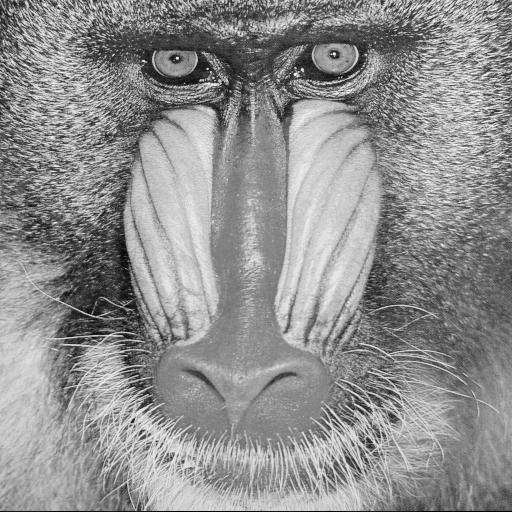
\includegraphics[scale=0.25]{results/original.png}
% \column{.5\textwidth}
% \centering
% 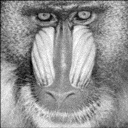
\includegraphics[scale=0.25]{results/noised.png}
% \end{columns}
% \end{frame}

% \begin{frame}{Results (with $(n_w, n_h) = (5, 5)$)}
% \centering
% \begin{columns}
% \column{.5\textwidth}
% \centering
% \includegraphics[scale=0.25]{results/bilateral/plot_mae.jpg}
% \column{.5\textwidth}
% \centering
% \includegraphics[scale=0.25]{results/bilateral/plot_mse.jpg}
% \end{columns}
% \end{frame}


% \begin{frame}{Results (with $(n_w, n_h) = (5, 5)$)}
% \centering
% \begin{columns}
% \column{.5\textwidth}
% \centering
% \includegraphics[scale=0.25]{results/bilateral/image_mae.jpg}
% \column{.5\textwidth}
% \centering
% \includegraphics[scale=0.25]{results/bilateral/image_mse.png}
% \end{columns}
% \end{frame}

\begin{frame}{Data}
\centering
\begin{columns}
\column{.5\textwidth}
\centering

\includegraphics[scale=0.25]{images/results/original.png}
\column{.5\textwidth}
\centering
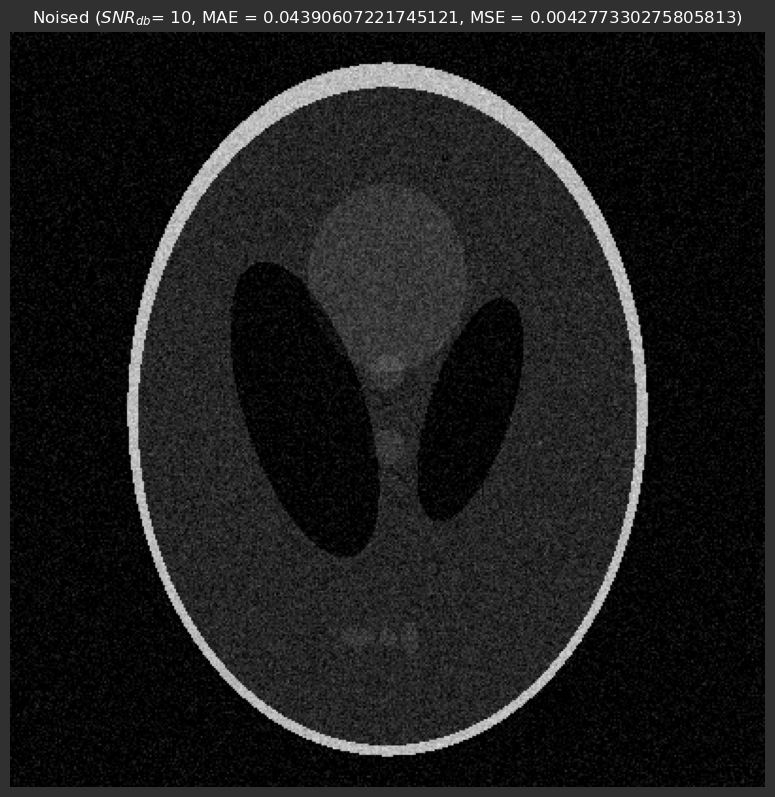
\includegraphics[scale=0.25]{images/results/noised.png}
\end{columns}
\end{frame}

\begin{frame}{Results (with $(n_w, n_h) = (5, 5)$)}
\centering
\begin{columns}
\column{.5\textwidth}
\centering
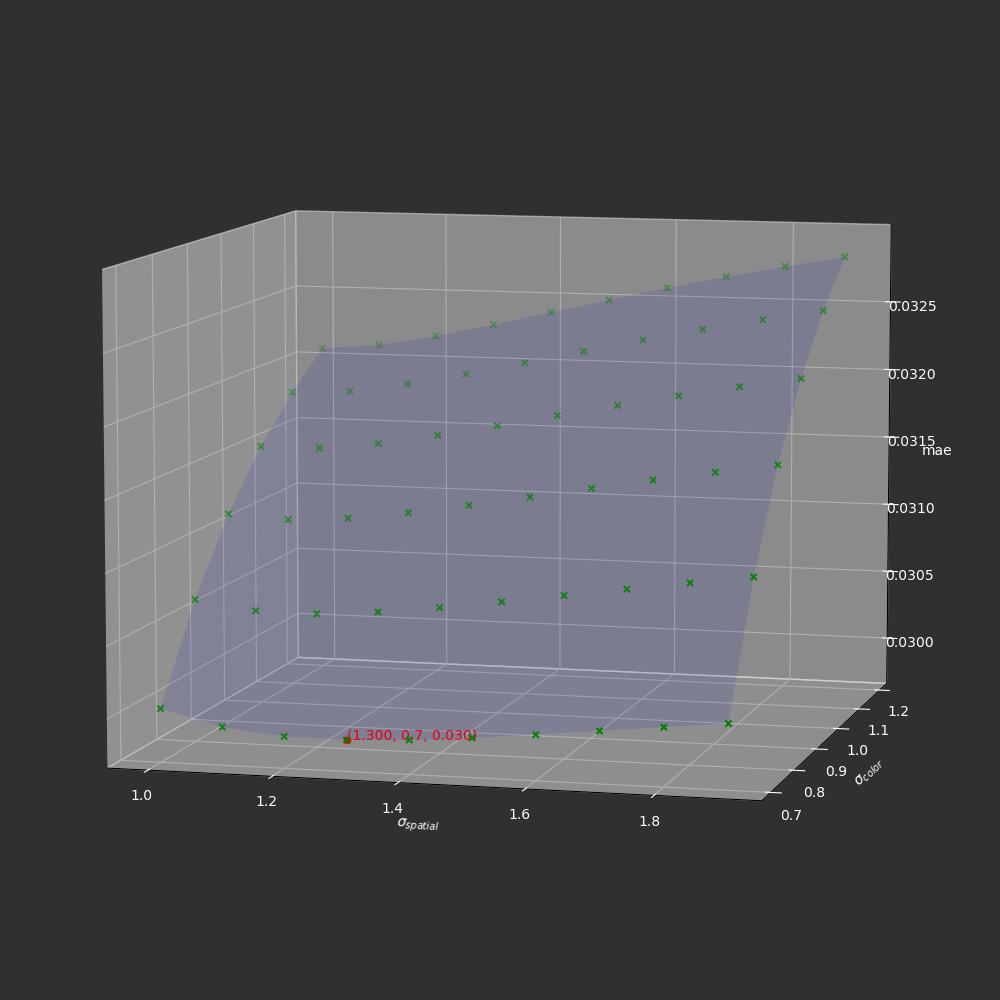
\includegraphics[scale=0.15]{images/results/bilateral/plot_mae.png}
\column{.5\textwidth}
\centering
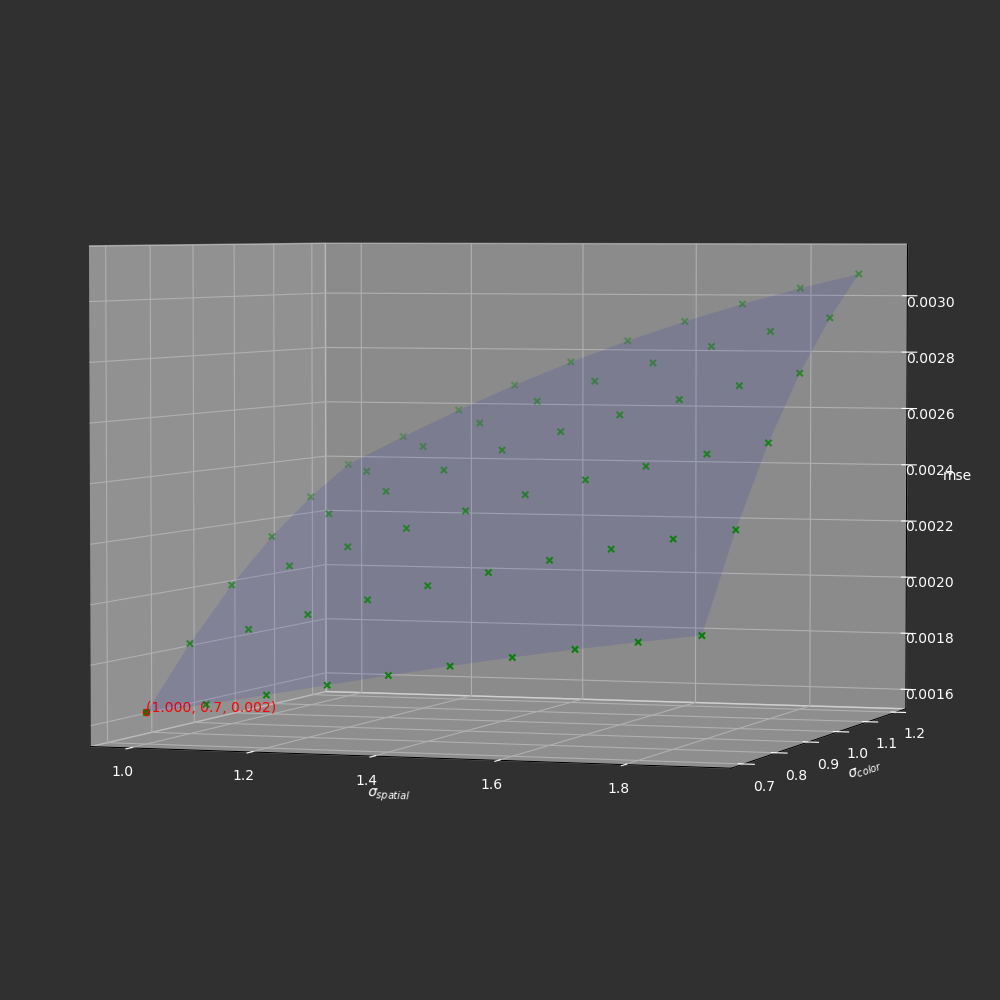
\includegraphics[scale=0.15]{images/results/bilateral/plot_mse.png}
\end{columns}
\end{frame}

\begin{frame}{Results (with $(n_w, n_h) = (5, 5)$)}
\centering
\begin{columns}
\column{.5\textwidth}
\centering
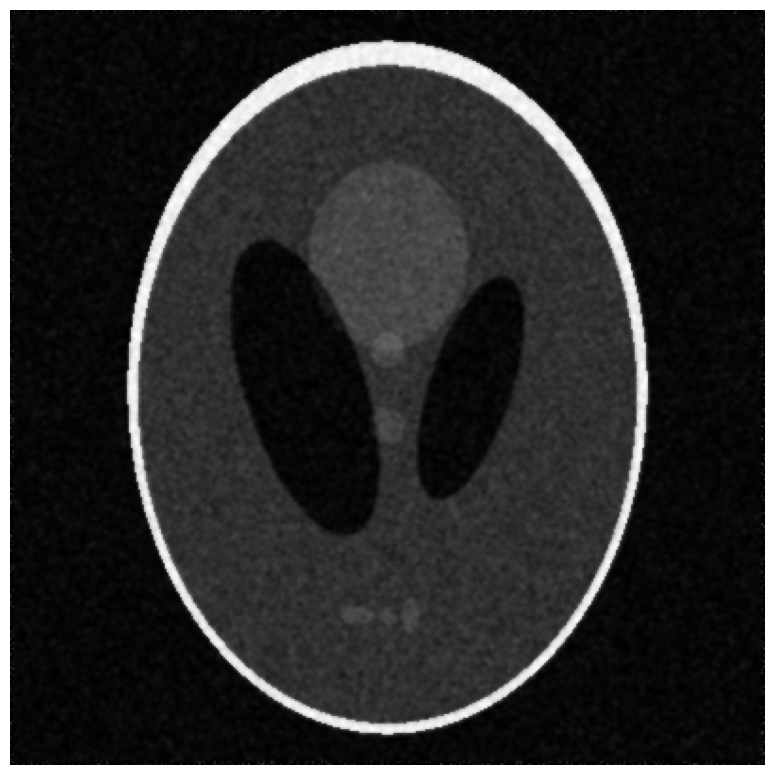
\includegraphics[scale=0.25]{images/results/bilateral/image_mae.png}
\column{.5\textwidth}
\centering
\includegraphics[scale=0.25]{images/results/bilateral/image_mse.png}
\end{columns}
\end{frame}


    \section{Anisotropic Filtering}
\frame{\sectionpage}

\begin{frame}{Principle}

\begin{itemize}
\item Iterative method
% \item Using knowledges about neighboors with derivation filters
\item \href{https://en.wikipedia.org/wiki/Partial_differential_equation}{PDE-based method}
\end{itemize}

\end{frame}

\begin{frame}{PDE meaning ?}
Partial Differential Equation (PDE): Differential equation with a function as solution
\end{frame}

\begin{frame}{Perona-Malik Model: Heat PDE}
\only<-2>{

\uncover<+->{

$\begin{cases}
I_{0} = I_\text{noisy} \\
I_{k+1} = I_{k} + \lambda [\sum\limits_{d \in Dir} 
(f_\text{diffusion} \circ (I_{k} \ast \nabla_{d}))] \\
\end{cases}$
}

\vspace{1cm}

\uncover<+->{
\begin{itemize}
\item $\lambda$ = hyper-parameter
\item $Dir = \left\lbrace \text{North}, \text{East}, \text{South}, \text{West} \right\rbrace$
\item $k$ = iteration number
\item $\nabla_{d}$ = derivation kernel with direction $d$
\item $f_\text{diffusion}$ = heat diffusion function
\end{itemize}
}

}

\end{frame}

\begin{frame}{Derivation kernels}
\begin{columns}

\column{.5\textwidth}
\centering
\begin{align*}
    \nabla_\text{North} = \begin{bmatrix} 0 & 1 & 0 \\ 0 & -1 & 0 \\ 0 & 0 & 0 \end{bmatrix}
\end{align*}
\begin{align*}
    \nabla_\text{South} = \begin{bmatrix} 0 & 0 & 0 \\ 0 & -1 & 0 \\ 0 & 1 & 0 \end{bmatrix}
\end{align*}

\column{.5\textwidth}
\centering
\begin{align*}
    \nabla_\text{West} = \begin{bmatrix} 0 & 0 & 0 \\ 1 & -1 & 0 \\ 0 & 0 & 0 \end{bmatrix}
\end{align*}
\begin{align*}
    \nabla_\text{Est} = \begin{bmatrix} 0 & 0 & 0 \\ 0 & -1 & 1 \\ 0 & 0 & 0 \end{bmatrix}
\end{align*}
\end{columns}

\end{frame}

\begin{frame}{Heat diffusion functions}

\only<-2>{

\uncover<+->{
$f_\text{diffusion} : \mathcal{R_{+}} \to \mathcal{R^{*}_{+}}$ such that
$\begin{cases}
f_\text{diffusion}(0) = 1 \\
\lim\limits_{u \to +\infty} f_\text{diffusion}(u) = 0
\end{cases}$
}

\vspace{1cm}
\uncover<+->{

Examples: \\

\begin{columns}

\column{.5\textwidth}
\centering
\begin{align*}
f_\text{diffusion}(u) = \frac{1}{1 + (\frac{u}{k})^{2}}
\end{align*}

\column{.5\textwidth}
\centering
\begin{align*}
f_\text{diffusion}(u) = e^{-(\frac{u}{k})^{2}}
\end{align*}

\end{columns}

\vspace{1cm}
with $k \in \mathcal{R^{*}_{+}}$
}
}

\end{frame}

\begin{frame}{Notation about $f_\text{diffusion} \circ (I_{k} \ast \nabla_{d})$}

Set $M = I_{k} \ast \nabla_{d}$.

\vspace{0.5cm}

\begin{align*}
f_\text{diffusion} \circ M
&= f_\text{diffusion} \circ \begin{bmatrix}
    m_{0, 0} & \dots & m_{0, M} \\
    \vdots & \ddots & \vdots \\
    m_{0, N} & \dots & m_{M, N}
\end{bmatrix} \\ 
&= \begin{bmatrix}
    f_\text{diffusion}(m_{0, 0}) & \dots & f_\text{diffusion}(m_{0, M}) \\
    \vdots & \ddots & \vdots \\
    f_\text{diffusion}(m_{0, N}) & \dots & f_\text{diffusion}(m_{M, N})
\end{bmatrix}
\end{align*}

\end{frame}

\begin{frame}{Algorithm}
\begin{algorithm}[H]
    \caption{Filtering Algorithm} % \label{euclid}
    \begin{algorithmic}[1]
        \Procedure{Denoising With Anisotropic Filter}{}\newline
        \textbf{Input:} $I$, $\lambda$, $N$ \\
        \textbf{Output:} $I_{N-1}$
        \State{$I_{0} = I$}
        \For{\texttt{$k \in [ 0, N [$}}
            \State{$I_{k+1} = I_{k} + \lambda [\sum\limits_{d \in Dir} 
(f_\text{diffusion} \circ (I_{k} \ast \nabla_{d}))]$}
        \EndFor
        \EndProcedure
    \end{algorithmic}
    % \label{alg_1}
\end{algorithm}
\end{frame}



% \begin{frame}{Results (with $N = 40$)}
% \centering
% \begin{columns}
% \column{.5\textwidth}
% \centering
% \includegraphics[scale=0.25]{results/anisotropic/plot_mae.jpg}
% \column{.5\textwidth}
% \centering
% \includegraphics[scale=0.25]{results/anisotropic/plot_mse.jpg}
% \end{columns}
% \end{frame}

% \begin{frame}{Results (with $N = 40$)}
% \centering
% \begin{columns}
% \column{.5\textwidth}
% \centering
% \includegraphics[scale=0.15]{results/anisotropic/image_mae.jpg}
% \column{.5\textwidth}
% \centering
% \includegraphics[scale=0.15]{results/anisotropic/image_mse.png}
% \end{columns}
% \end{frame}

\begin{frame}{Data}
\centering
\begin{columns}
\column{.5\textwidth}
\centering

\includegraphics[scale=0.25]{images/results/original.png}
\column{.5\textwidth}
\centering
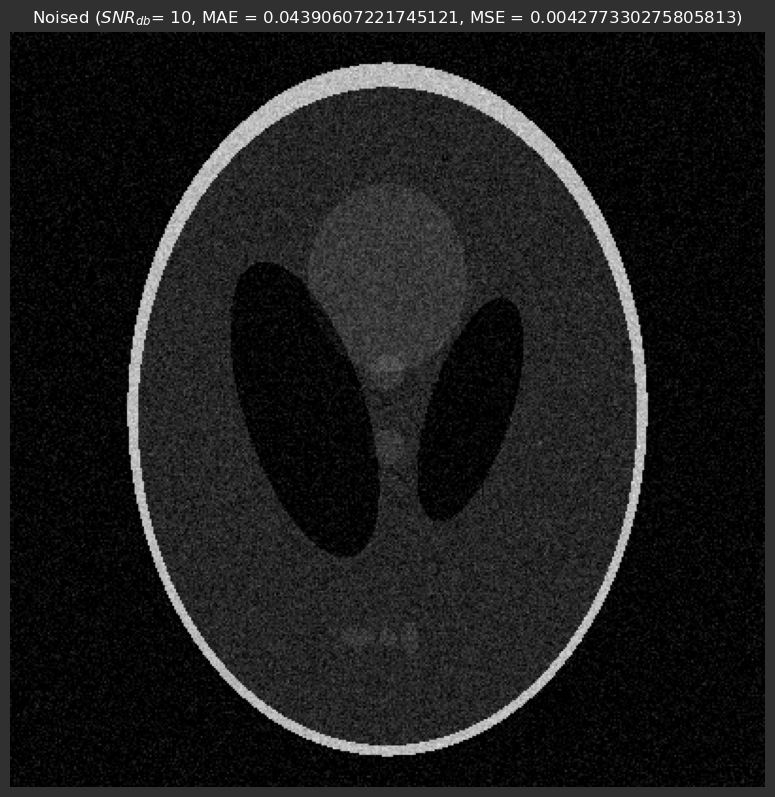
\includegraphics[scale=0.25]{images/results/noised.png}
\end{columns}
\end{frame}

\begin{frame}{Results (with $N = 40$)}
\centering
\begin{columns}
\column{.5\textwidth}
\centering
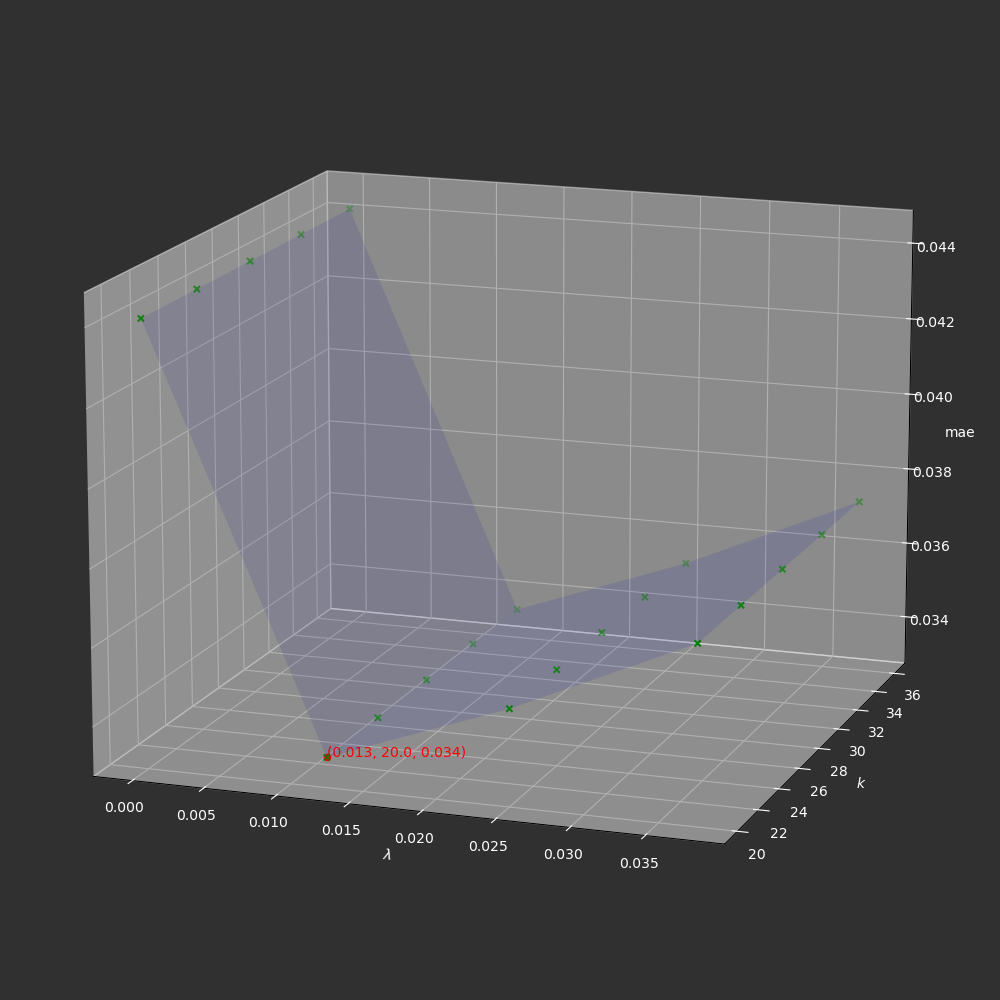
\includegraphics[scale=0.15]{images/results/anisotropic/plot_mae.png}
\column{.5\textwidth}
\centering
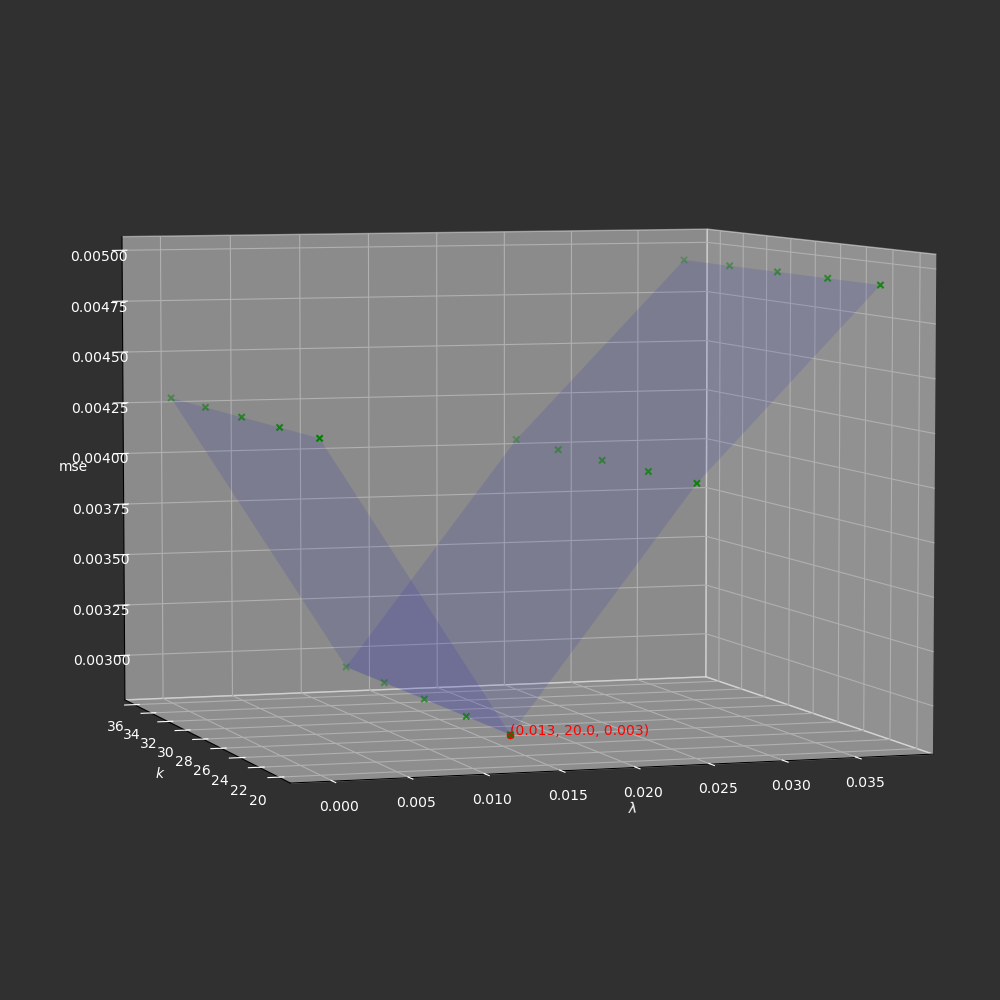
\includegraphics[scale=0.15]{images/results/anisotropic/plot_mse.png}
\end{columns}
\end{frame}

\begin{frame}{Results (with $N = 40$)}
\centering
\begin{columns}
\column{.5\textwidth}
\centering
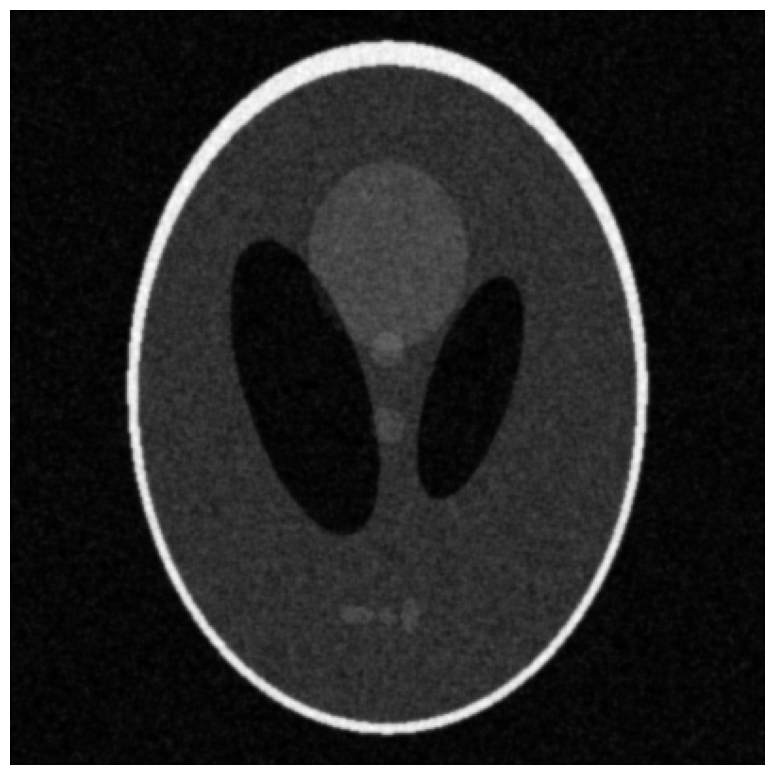
\includegraphics[scale=0.25]{images/results/anisotropic/image_mae.png}
\column{.5\textwidth}
\centering
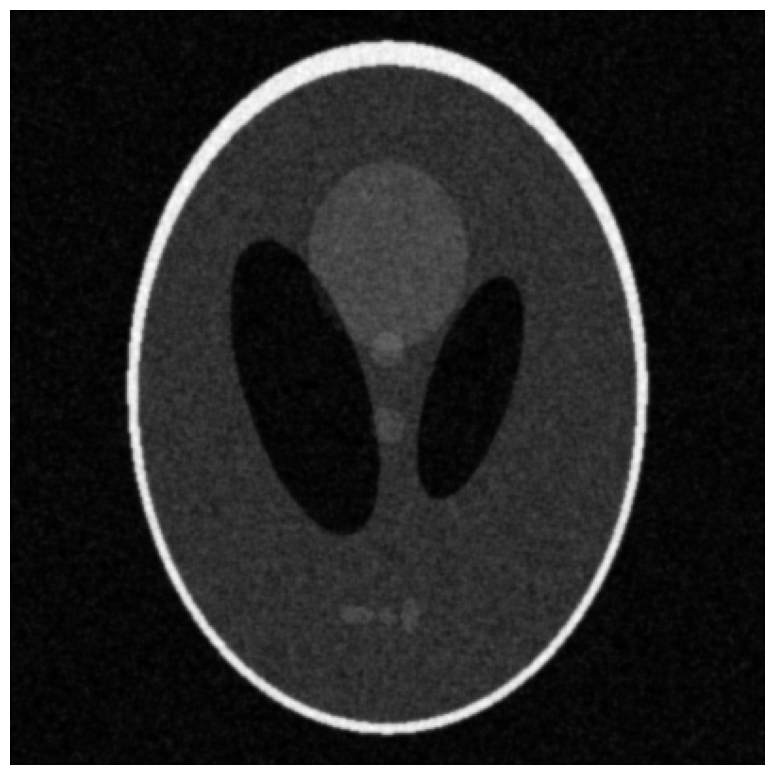
\includegraphics[scale=0.25]{images/results/anisotropic/image_mse.png}
\end{columns}
\end{frame}
    % \section{Block-matching and 3D filtering (BM3D)}
\frame{\sectionpage}

\begin{frame}{Principle}

\begin{itemize}
    \item Iterative method
    \item Using knowledge about neighbors
    \item Grouping patches with a "similarity" measure
\end{itemize}

\end{frame}

\begin{frame}{Approach}
\begin{itemize}
    \item Split image into overlapping tiles
    \item Group tiles by their pairwise structural similarity
    \item Perform 3D "naive" denoising on each stacked block
    \item Return each block to their original place on the image
\end{itemize}
\end{frame}

% \begin{frame}{Algorithm}
% \begin{algorithm}[H]
%     \caption{Filtering Algorithm} % \label{euclid}
%     \begin{algorithmic}[1]
%         \Procedure{Denoising With BM3D}{}\newline
%         \textbf{Input:} $I$, $\sigma_{spatial}$, $threshold$ \\
%         \textbf{Output:} $I_{D}$
%         \State{$patch_list = list()$}
%         \For{$patch \in \text{windows}\left(I\right)$}
%             \State{$patches = list()$}
%             \For{$other_path \in \text{windows}\left(I\right)$}
%                 \State{$similarity = \text{SSIM}\left(path, other_patch\right)$}
%                 \If{$similarity > threshold$}
%                     \State{$\text{insert}\left(other_patch\right)$}
%                 \EndIf
%             \EndFor
%             \State{$\text{insert}\left(patch_list, patches\right)$}
%         \EndFor
%         \For{$patches \in patch_list$}
%             % \State{$sparse = \text{transform_sparse}\left(patches\right)$}
%             % \State{$sparse = \text{thresholding}\left(sparse\right)$}
%             % \State{$sparse = \text{transform_sparse_inv}\left(patches\right)$}
%             % \For{$patch \in sparse$}
%             %     \State{$\text{place_into}\left(I_D, patch\right)$}
%             % \EndFor
%         \EndFor
%         \EndProcedure
%     \end{algorithmic}
%     % \label{alg_1}
% \end{algorithm}
% \end{frame}

\begin{frame}{Data}
\centering
\begin{columns}
\column{.5\textwidth}
\centering

\includegraphics[scale=0.25]{images/results/original.png}
\column{.5\textwidth}
\centering
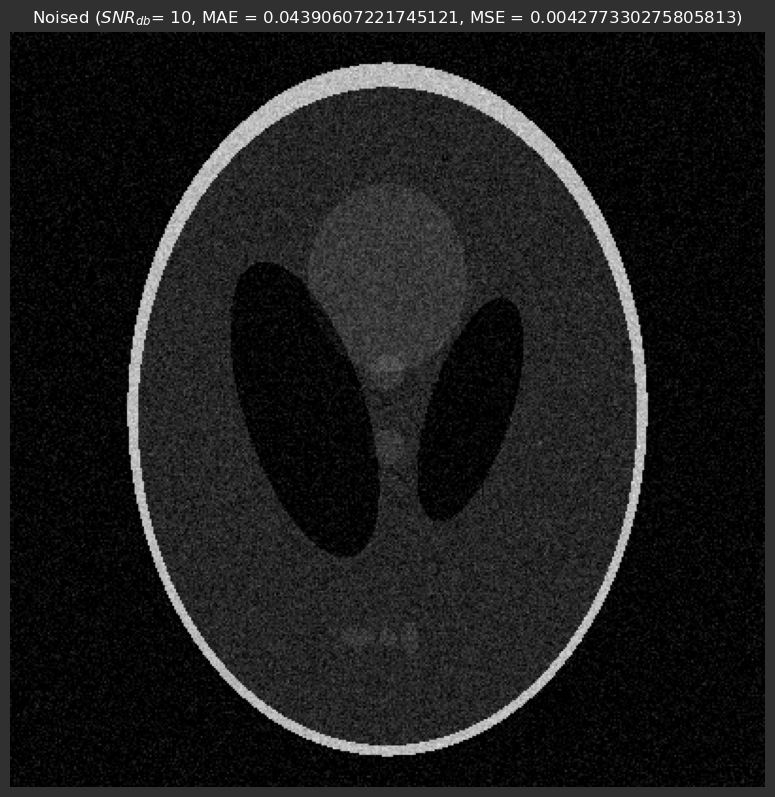
\includegraphics[scale=0.25]{images/results/noised.png}
\end{columns}
\end{frame}

\begin{frame}{Results}
\centering
\begin{columns}
\column{.5\textwidth}
\centering
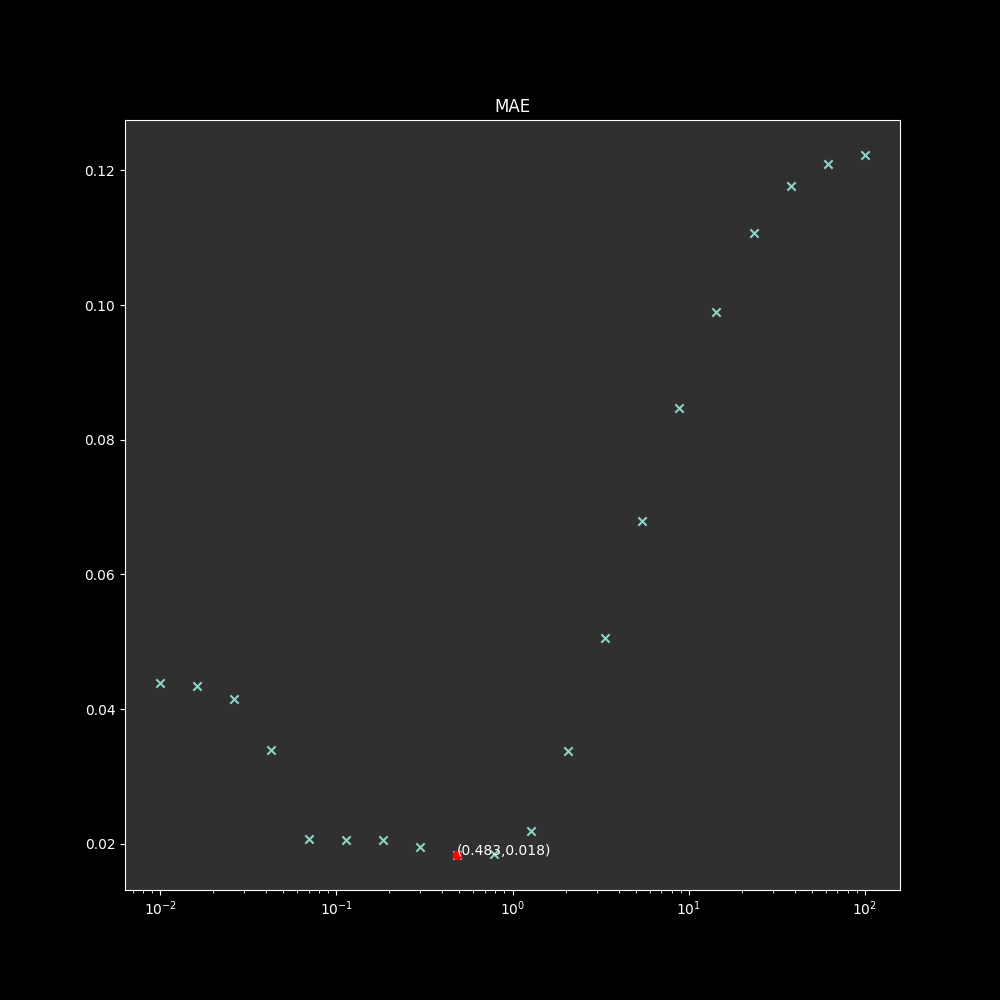
\includegraphics[scale=0.25]{images/results/bm3d/bm3d_mae.png}
\column{.5\textwidth}
\centering
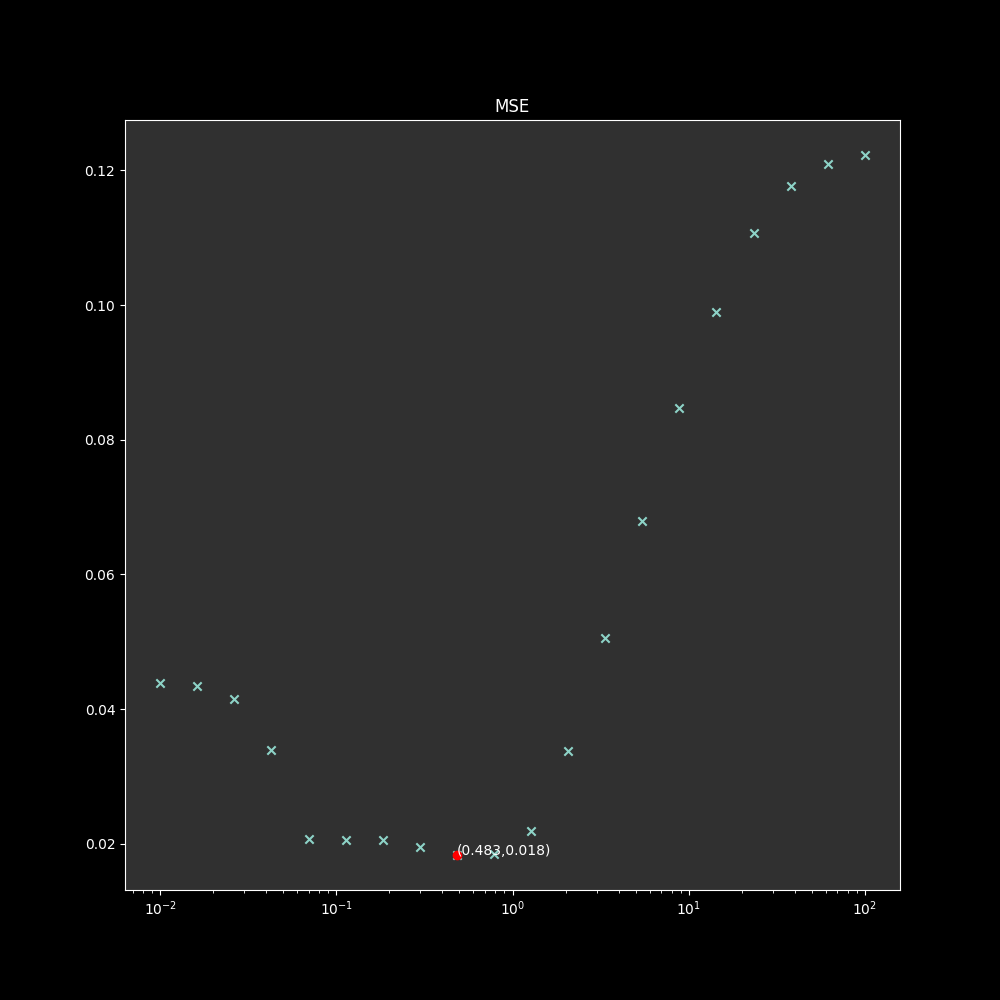
\includegraphics[scale=0.25]{images/results/bm3d/bm3d_mse.png}
\end{columns}
\end{frame}

\begin{frame}{Results (min sigma 0.483)}
\centering
\centering
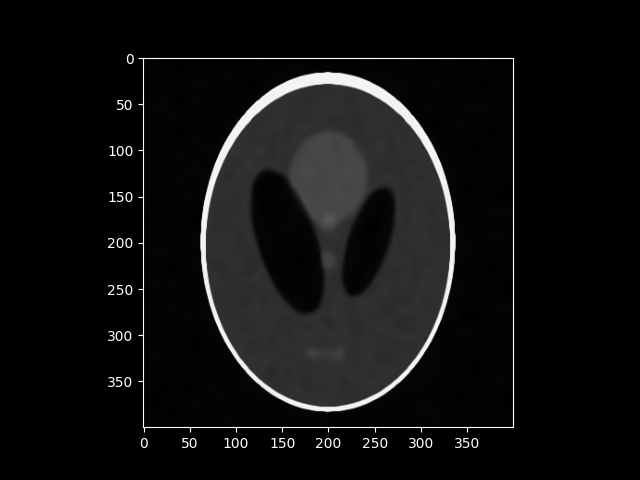
\includegraphics[scale=0.6]{images/results/bm3d/bm3d_best.png}
\end{frame}


    % \section{Autoencoder}
\frame{\sectionpage}

\begin{frame}{Principle}

\begin{itemize}
\item Deep-learning method
\item Approach based on learning the noise density and PSF
\end{itemize}

\end{frame}

\begin{frame}{Approach}
\begin{itemize}
    \item Take N convolutions progressively increasing the number of channels
    \item Linearize the CNN section and reduce the size to create the bottleneck
    \item Flip the encoder section around to recreate the image
\end{itemize}
\end{frame}

\begin{frame}{Problems}
\begin{itemize}
    \item Having to learn hyper-parameters from a training set implies specialization
    \item Difficulty to make the model resolution-independent
    \item Computationally (and resourcefully) expensive to train
\end{itemize}
\end{frame}
    % \section{Results}
\frame{\sectionpage}

% \begin{frame}{Principle}

% \begin{itemize}
%     \item Iterative method
%     \item Using knowledges about neighboors
%     \item Grouping patches with "similarity" measure
% \end{itemize}

% \end{frame}
    
    % \section{Fourier's Physics Playground}

    \subsection{Maxwell's Electrodynamics}
    \frame{\sectionpage}

    \begin{frame}{In the beggining, God said:}
        \begin{equation*}
            \left\lbrace
            \begin{aligned}
                &\div{\vb{E}} = \frac{\rho}{\e}\\
                &\div{\vb{B}} = 0\\
                &\curl{\vb{E}} = - \pdv{\vb{B}}{t}\\
                &\curl{\vb{B}} = \m\vb{J}
 + \m\e\pdv{\vb{E}}{t}                        
            \end{aligned}
            \right.
        \end{equation*}
        
        \uncover<2>{and there was light!}
    \end{frame}
    
    \begin{frame}{Too hard, let's try something different}
        \begin{equation*}
            \left\lbrace
            \begin{aligned}
                &\vb{E} = - \grad{V} - \pdv{\vb{A}}{t} \\
                &\vb{B} = \curl{\vb{A}}
            \end{aligned}
            \right.
        \end{equation*}
    \end{frame}
    
    \begin{frame}{Wave Equations}
        \begin{equation*}
            \left\lbrace
            \begin{aligned}
                &\laplacian{V} - \frac{1}{c^2}\pdv[2]{V}{t} = - \frac{\rho}{\e}\\
                &\laplacian{\vb{A}} - \frac{1}{c^2}\pdv[2]{\vb{A}}{t} = - \m\vb{J}
            \end{aligned}
            \right.
        \end{equation*}
    \end{frame}
    
    \begin{frame}{All Wave Equations In One}
        \begin{equation*}
            \laplacian{\psi(\vb{r},t)} - \frac{1}{c^2}\pdv[2]{\psi}{t} (\vb{r},t) = - g(\vb{r},t)
        \end{equation*}
    \end{frame}
    
    \begin{frame}{Fourier's Opinion}
        \begin{equation*}
            \widehat{g}(\vb{r},\omega) = \frac{1}{\sqrt{2\pi}} \int_{-\infty}^{+\infty} g(\vb{r},t) e^{-i\omega t} \dd{t}
        \end{equation*}
        
        \begin{equation*}
            g(\vb{r},t) = \frac{1}{\sqrt{2\pi}} \int_{-\infty}^{+\infty} \widehat{g}(\vb{r},\omega) e^{i\omega t} \dd{\omega}
        \end{equation*}
    \end{frame}
    
    \begin{frame}{Fourier's Opinion}
        \begin{equation*}
            \widehat{\psi}(\vb{r},\omega) = \frac{1}{\sqrt{2\pi}} \int_{-\infty}^{+\infty} \psi(\vb{r},t) e^{-i\omega t} \dd{t}
        \end{equation*}
        
        \begin{equation*}
            \psi(\vb{r},t) = \frac{1}{\sqrt{2\pi}} \int_{-\infty}^{+\infty} \widehat{\psi}(\vb{r},\omega) e^{i\omega t} \dd{\omega}
        \end{equation*}
    \end{frame}
    
    \begin{frame}{Fourier's Opinion}
        \begin{equation*}
            \laplacian{\psi(\vb{r},t)} - \frac{1}{c^2}\pdv[2]{\psi}{t} (\vb{r},t) = - g(\vb{r},t)
        \end{equation*}
        
        \begin{equation*}
            \laplacian{\widehat{\psi}(\vb{r},\omega)} + \frac{\omega^2}{c^2} \widehat{\psi}(\vb{r},\omega) = - \widehat{g}(\vb{r},\omega)
        \end{equation*}
    \end{frame}
    
    \begin{frame}{Green Function}
        \uncover<+->{\begin{equation*}
            L \phi(\vb{r}) = - s(\vb{r})
        \end{equation*}}
        
        \uncover<+->{\begin{equation*}
            L G(\vb{r} - \vb{r'}) = - \dirac{\vb{r} - \vb{r'}}
        \end{equation*}}
        
        \uncover<+->{\begin{equation*}
            \phi(\vb{r}) = \int G(\vb{r} - \vb{r'}) s(\vb{r'}) \dd{\tau'}
        \end{equation*}}
        
        \uncover<+->{\begin{equation*}
            L \phi(\vb{r}) = \int L G(\vb{r} - \vb{r'}) s(\vb{r'}) \dd{\tau'} =  - \int \dirac{\vb{r} - \vb{r'}} s(\vb{r'}) \dd{\tau'} = -s(\vb{r})
        \end{equation*}}
    \end{frame}
    
    \begin{frame}{One At a Time}
        \uncover<+->{\begin{equation*}
            \laplacian{\widehat{\psi}(\vb{r},\omega)} + \frac{\omega^2}{c^2} \widehat{\psi}(\vb{r},\omega) = - \widehat{g}(\vb{r},\omega)
        \end{equation*}}
        
        \uncover<+->{\begin{equation*}
            \laplacian{G(\vb{r} - \vb{r'})} + \frac{\omega^2}{c^2} G(\vb{r} - \vb{r'}) = - \dirac{\vb{r} - \vb{r'}}
        \end{equation*}}
    \end{frame}
    
    \begin{frame}{Solution for $\vb{r} - \vb{r'} \neq \vb{0}$}
        \uncover<+->{\begin{equation*}
            \frac{1}{r}\dv[2]{(rG)}{r} + k^2 G = 0
        \end{equation*}}
        
        \uncover<+->{\begin{equation*}
            G(r) = \frac{A}{r}e^{\pm i k r}
        \end{equation*}}
    \end{frame}
    
    \begin{frame}{Recovering $0$ Psychological Trauma}
        \uncover<+->{\begin{equation*}
            \laplacian{G(\vb{r} - \vb{r'})} + \frac{\omega^2}{c^2} G(\vb{r} - \vb{r'}) = - \dirac{\vb{r} - \vb{r'}}
        \end{equation*}}
        
        \uncover<+->{\begin{equation*}
            A \int \laplacian{\frac{1}{r}} \dd{\tau'} + 4\pi A \frac{\omega^2}{c^2} \int \frac{r^2}{r} \dd{r}  = - \int \dirac{\vb{r} - \vb{r'}} \dd{\tau'}
        \end{equation*}}
        
        \uncover<+->{\begin{equation*}
            - 4 \pi A  = - 1
        \end{equation*}}
    \end{frame}
    
    \begin{frame}{Back To Our Problem}
        \uncover<+->{\begin{equation*}
            \widehat{\psi}(\vb{r}, \omega) = \int G(\rc)\widehat{g}(\vb{r'}, \omega) \dd{\tau'}
        \end{equation*}}
        
        \uncover<+->{\begin{equation*}
            G(\rc) = \frac{1}{4\pi \rc}e^{\pm i k \rc}
        \end{equation*}}
        
        \uncover<+->{\begin{equation*}
            \widehat{\psi}(\vb{r}, \omega) = \frac{1}{4\pi} \int \frac{\widehat{g}(\vb{r'}, \omega) e^{\pm i k \rc}}{\rc} \dd{\tau'}
        \end{equation*}}
    \end{frame}
    
    \begin{frame}{Actually Solving Our Problem}
        \uncover<+->{\begin{equation*}
            \psi(\vb{r},t) = \frac{1}{\sqrt{2\pi}} \int_{-\infty}^{+\infty} \widehat{\psi}(\vb{r},\omega) e^{i\omega t} \dd{\omega}
        \end{equation*}}
            
        \uncover<+->{\begin{equation*}
            \psi(\vb{r},t) = \frac{1}{4 \pi \sqrt{2\pi}} \iint \frac{\widehat{g}(\vb{r'}, \omega) e^{i \omega t \pm i \omega \frac{\rc}{c}}}{\rc} \dd{\omega} \dd{\tau'}
        \end{equation*}}
    \end{frame}
    
    \begin{frame}{Actually Solving Our Problem}
        \uncover<+->{\begin{equation*}
            \psi(\vb{r},t) = \frac{1}{4 \pi \sqrt{2\pi}} \iint \frac{\widehat{g}(\vb{r'}, \omega) e^{i \omega \prnt{t \pm \frac{\rc}{c}}}}{\rc} \dd{\omega} \dd{\tau'}
        \end{equation*}}
        
        \uncover<+->{\only<-2>{\begin{equation*}
            \psi(\vb{r},t) = \frac{1}{4 \pi} \int \frac{g(\vb{r'}, t \pm \frac{\rc}{c})}{\rc} \dd{\tau'}
        \end{equation*}}
        
        \only<3>{\begin{equation*}
            \psi(\vb{r},t) = \frac{1}{4 \pi} \int \frac{g(\vb{r'}, t - \frac{\rc}{c})}{\rc} \dd{\tau'}
        \end{equation*}}}
    \end{frame}
    
    \begin{frame}{Back at Maxwell's}
        \begin{equation*}
            V(\vb{r},t) = \frac{1}{4 \pi \e} \int \frac{\rho(\vb{r'}, t - \frac{\rc}{c})}{\rc} \dd{\tau'}
        \end{equation*}
        
        \begin{equation*}
            \vb{A}(\vb{r},t) = \frac{\m}{4 \pi} \int \frac{\vb{J}(\vb{r'}, t - \frac{\rc}{c})}{\rc} \dd{\tau'}
        \end{equation*}
    \end{frame}
    
    \begin{frame}{One Last Step} 
        \begin{equation*}
            \left\lbrace
            \begin{aligned}
                &\vb{E} = - \grad{V} - \pdv{\vb{A}}{t} \\
                &\vb{B} = \curl{\vb{A}}
            \end{aligned}
            \right.
        \end{equation*}
    \end{frame}
    
    \begin{frame}{Jefimenko Equations}
        \begin{equation*}
            \vb{E}(\vb{r},t) = \frac{1}{4\pi\e}\int \frac{\hrc}{\rc^2}\rtd{\rho} + \frac{\hrc}{c\rc} \rtd{\pdv{\rho}{t}} - \frac{1}{c^2\rc} \rtd{\pdv{\vb{J}}{t}} \dd{\tau'}
        \end{equation*}
                    
        \begin{equation*}
            \vb{B}(\vb{r},t) = \frac{\m}{4\pi}\int \prnt{\frac{1}{\rc^2} \rtd{\vb{J}} + \frac{1}{c\rc} \rtd{\pdv{\vb{J}}{t}}} \cp \hrc \dd{\tau'}
        \end{equation*}
    \end{frame}
    
    \subsection{Heisenberg's Uncertainty Principle}
    \frame{\sectionpage}
    \begin{frame}{Position and Momentum}
        \uncover<+->{\begin{equation*}
            \psi(x) = \bra{x}\ket{\psi} = \int \bra{x}\ket{k} \bra{k}\ket{\psi} \dd{k} = \frac{1}{\sqrt{2\pi}} \int e^{ikx} \psi(k) \dd{k}
        \end{equation*}}
        
        \uncover<+->{\begin{equation*}
            \psi(k) = \bra{k}\ket{\psi} = \int \bra{k}\ket{x} \bra{x}\ket{\psi} \dd{x} = \frac{1}{\sqrt{2\pi}} \int e^{-ikx} \psi(x) \dd{x}
        \end{equation*}}
    \end{frame}
    
    \begin{frame}{Position and Momentum (but weirder)}
        \uncover<+->{\begin{equation*}
            \left\lbrace
            \begin{aligned}
                &X\ket{\psi} = x \psi(x) \\
                &K \ket{\psi} = - i \pdv{\psi}{x} (x)
            \end{aligned}
            \right.
        \end{equation*}}
        
        \uncover<+->{\begin{equation*}
            \left\lbrace
            \begin{aligned}
                &X\ket{\psi} = - i \pdv{\psi}{k} (k) \\
                &K \ket{\psi} = k \psi(k)
            \end{aligned}
            \right.
        \end{equation*}}
    \end{frame}
    
    \begin{frame}{Fourier Diplomacy}
        \uncover<+->{\begin{equation*}
            \ket{x} \xleftrightarrow[\mathcal{F}^{-1}]{\mathcal{F}} \ket{k}
        \end{equation*}}
    \end{frame}
    
    \begin{frame}{Fourier Uncertainty}
        \begin{enumerate}
            \item<+-> $\psi(x):$ what is $x$?
            \item<+-> $\psi(k):$ what is $k$?
        \end{enumerate}
    \end{frame}
    
    \begin{frame}{Definite Position}
        \begin{equation*}
            \psi(x) = \sqrt{\frac{\pi}{2}}\prnt{\dirac{x-x_0} + \dirac{x+x_0}}    
        \end{equation*}
        
        \centering 
        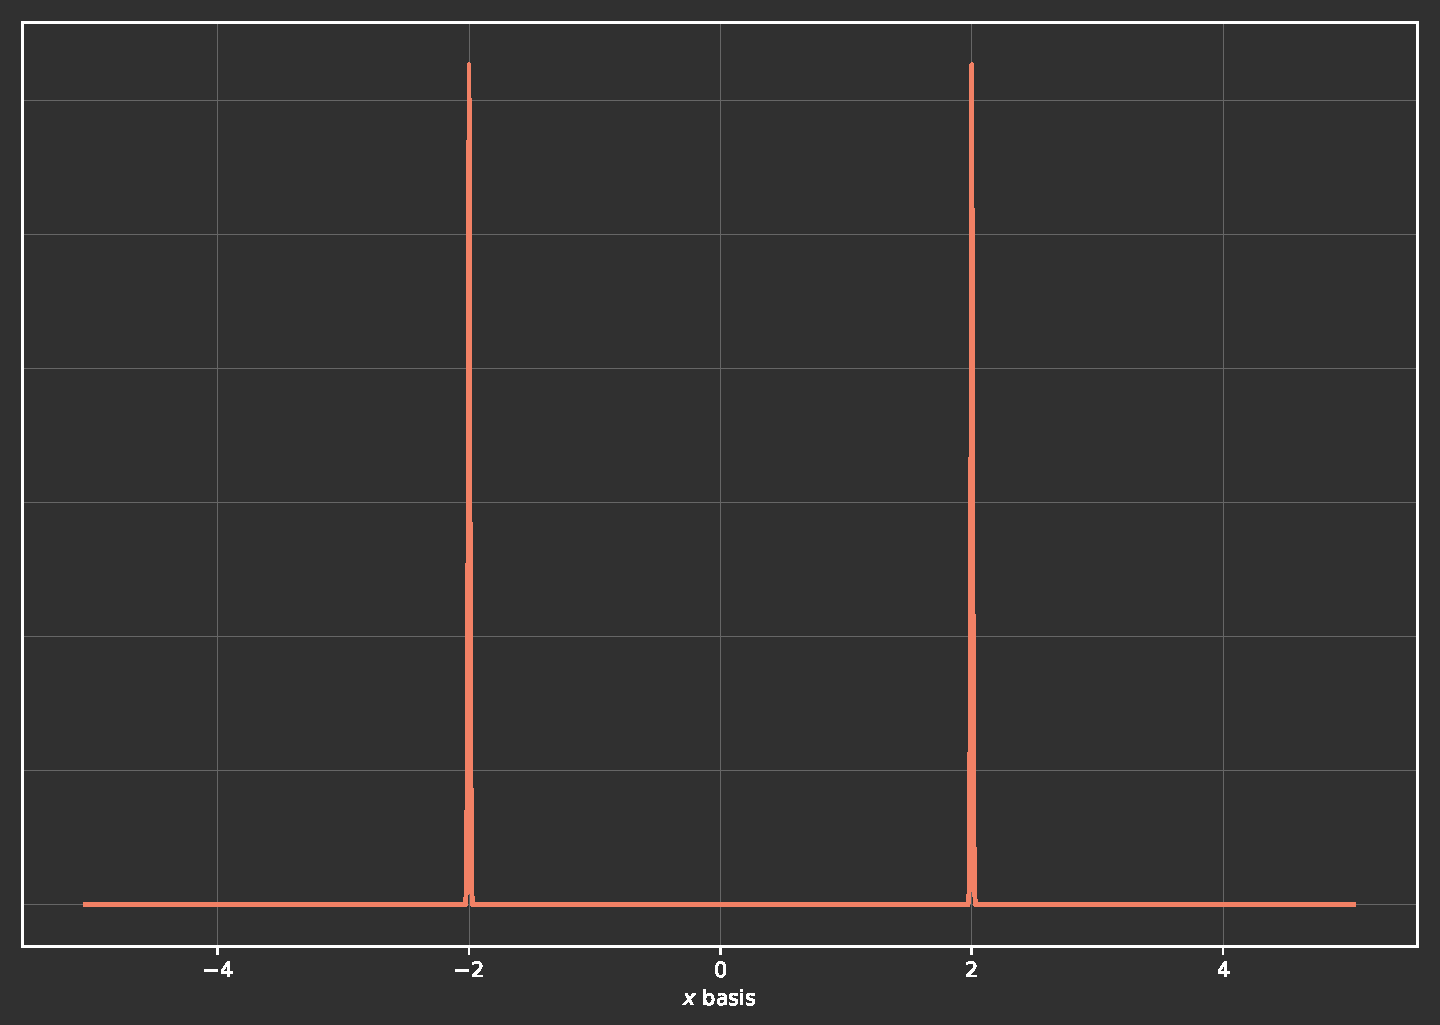
\includegraphics[height = 0.65 \textheight]{images/Pulse3-Fourier.pdf}
    \end{frame}
    
    \begin{frame}{Undefinite Momentum}
        \begin{equation*}
            \psi(k) = \cos(x_0 k) 
        \end{equation*}
        
        \centering
        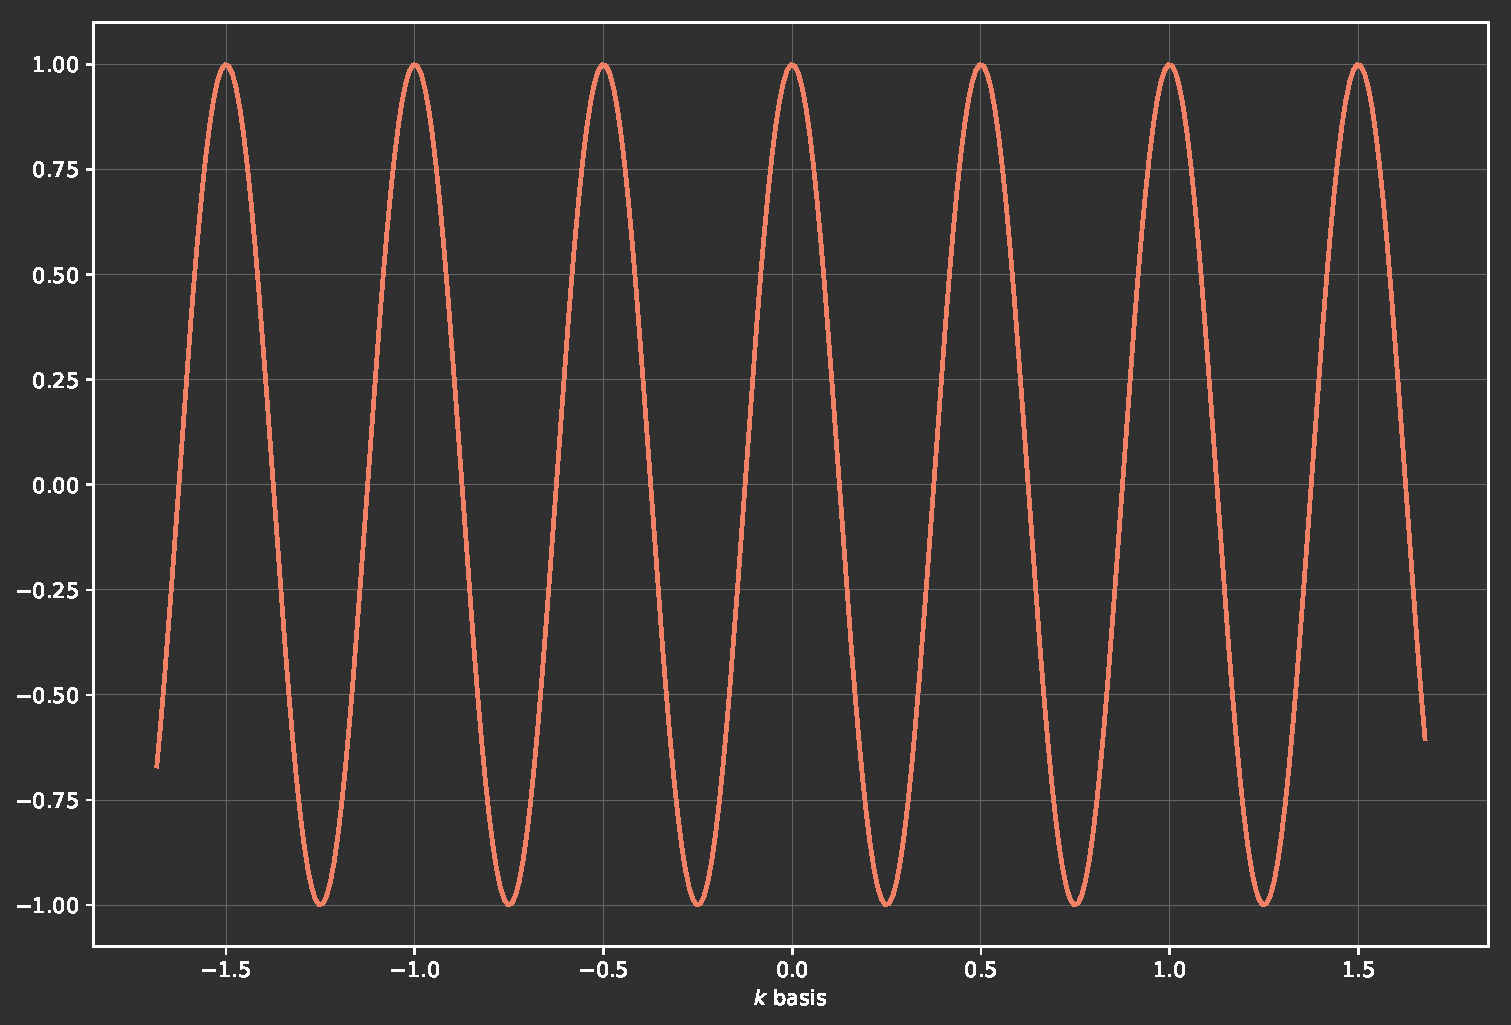
\includegraphics[height = 0.65 \textheight]{images/Pulse3.pdf}
    \end{frame}
    
    \begin{frame}{Uncertainty Relation}
        \begin{block}{\centering$\sigma_x\sigma_p \geq \frac{\hbar}{2}$}
            The uncertainty relation is a consequence of the general fact that anything narrow in one space is wide in the transform space and vice versa. So if you are a 45 kg weakling and are taunted by a 270 kg bully, just ask him to step into momentum space!
        
            \alert{Ramamurti Shankar}
        \end{block}
    \end{frame}
    
    % \section*{Acknowledgments} %You can remove this if you do not want to use it
    %     \begin{frame}{Acknowledgments}
    %         The author is extremely thankful to Prof. Antônio F. R. T. Piza for the short, yet wonderful, conversations about this seminar.
    %     \end{frame}
    
    % \section*{References} %You can remove this if you do not want to use it
    %     \nocite{Djairo} \nocite{PhilPanof} \nocite{Fleming} \nocite{Shankar}
    %     \begin{frame}{References}
    %         \printbibliography
    %     \end{frame}

    % \section{}
    \begin{frame}{}
        \centering
            \Huge\bfseries
        \textcolor{orange}{The End}
    \end{frame}
\end{document}
